\subsection{Team 3}
\label{app:team3}

\paragraph{Data} The challenge training (\chk{2,992} scans) and validation
(\chk{200} scans) sets. External data were \chk{8,000} sentence--mask pairs from
CT-RATE \citep{hamamci2026generalist}, with pseudo-masks of nodules and effusions
from TotalSegmentator \citep{wasserthal2023totalsegmentator}, used by two
ensemble members (one of them only the \chk{1,540} effusion pairs). In-house data
were used only for the pretraining of TAP-CT \citep{veenboer2025tap}
(\chk{105,000} CT volumes). Pretrained weights were VoxTell v1.1
\citep{rokuss2026voxtell}, Qwen3-Embedding \citep{zhang2025qwen3}, TAP-CT-B-3D
and Qwen2.5-7B \citep{yang2025qwen3}. Derived data were TotalSegmentator lobe
masks, a lobe mapping of all finding sentences by Qwen3-32B
\citep{yang2025qwen3}, synonym-based text augmentation and Qwen2.5 paraphrases.
Test-set exposure: the CT-RATE pool incidentally included test studies, so one
member saw \chk{80} of the \chk{300} test studies and another \chk{10} of these,
as image, report sentence and pseudo-mask, but never the challenge masks or
sentences. Retraining both members with these studies replaced by other CT-RATE
scans changed the final masks equally on exposed and unexposed studies (Dice
\chk{0.976} vs.\ \chk{0.974} between versions).

\paragraph{Pre-processing} VoxTell members use the native grid, z-scored
intensities and random $192^3$ crops, one third of them centred on a finding.
TAP-CT resamples to 1.5\,mm isotropic voxels, clips to $[-1008, 822]$\,HU,
z-scores, and uses $24 \times 224 \times 224$ crops.

\paragraph{Architecture and text encoder} VoxTell: an nnU-Net residual encoder
\citep{isensee2021nnu,isensee2024nnu} and a transformer decoder in which the
frozen Qwen3-Embedding-4B sentence embedding queries the $12^3$ bottleneck tokens
(440M trainable parameters). TAP-CT: a 3D ViT-B (87M parameters) conditioned on
Qwen3-Embedding-0.6B through FiLM \citep{perez2018film}, followed by a
convolutional decoder.

\paragraph{Training} VoxTell members were trained from VoxTell v1.1 for 250
epochs, five of them for up to 430, with deeply supervised Dice plus
cross-entropy loss (Tversky loss in three members), SGD at $10^{-4}$ with
polynomial decay, and a batch size of 8, taking about 7\,h per 250 epochs on one
H100. There was no image augmentation, and text augmentation replaced phrases
with equivalent phrasings seen in the data ($p = 0.5$). The validation data were
in every member's training set. TAP-CT members used Dice plus cross-entropy,
AdamW and a batch size of 16, with 50,000 steps with the encoder frozen followed
by 25,000 steps of fine-tuning (4.5\,h per seed on one H100), five seeds,
left--right flips, paraphrases and negatives with swapped locations.

\paragraph{Ensembling} The probability maps of twelve VoxTell members, which
differ in initialization, loss, sampling and auxiliary data, are averaged and
fused 0.8/0.2 with the mean of five TAP-CT seeds (Figure~\ref{fig:app-team3}).

\paragraph{Post-processing} The fused map is restricted to the named lobe
(dilated by 16 voxels) or lung (12 voxels), thresholded per finding by a
gradient-boosted regressor, and cleaned by a small 3D CNN that removes components
predicted to lower Dice (both fitted on the validation set). Voxels claimed by
several findings go to the most confident one. The only language model used at
inference is the Qwen3-32B lobe mapping.

\paragraph{Inference time and hardware} On one H100, a VoxTell member takes
3.7\,min per scan for all findings jointly, about 24 GPU-minutes per finding for
the twelve members, and the five TAP-CT seeds together take 23\,s per scan.

\paragraph{Final submission and lessons} The final submission was TAGS\_TAPv3
(full test set Dice \chk{0.362}). Most helpful were TAP-CT as a second
architecture, the dilated lobe restriction and the per-finding thresholds.
Changes targeting location words, pseudo-labels and extra public data did not
help. Four late post-processing additions each gained 0.001--0.004 on the
validation set and the public half, yet the submission without them scored
\chk{0.365} on the full test set.

\paragraph{Code and weights} Code:
\url{https://github.com/nki-radiology/TAGS-ReXGroundingCT} (Apache-2.0).
Weights of all members: \url{https://huggingface.co/fomofo/TAGS-ReXGroundingCT}
(CC BY-NC-SA 4.0, TAP-CT seeds CC BY-NC 4.0).

\begin{figure*}[!htbp]
\centering
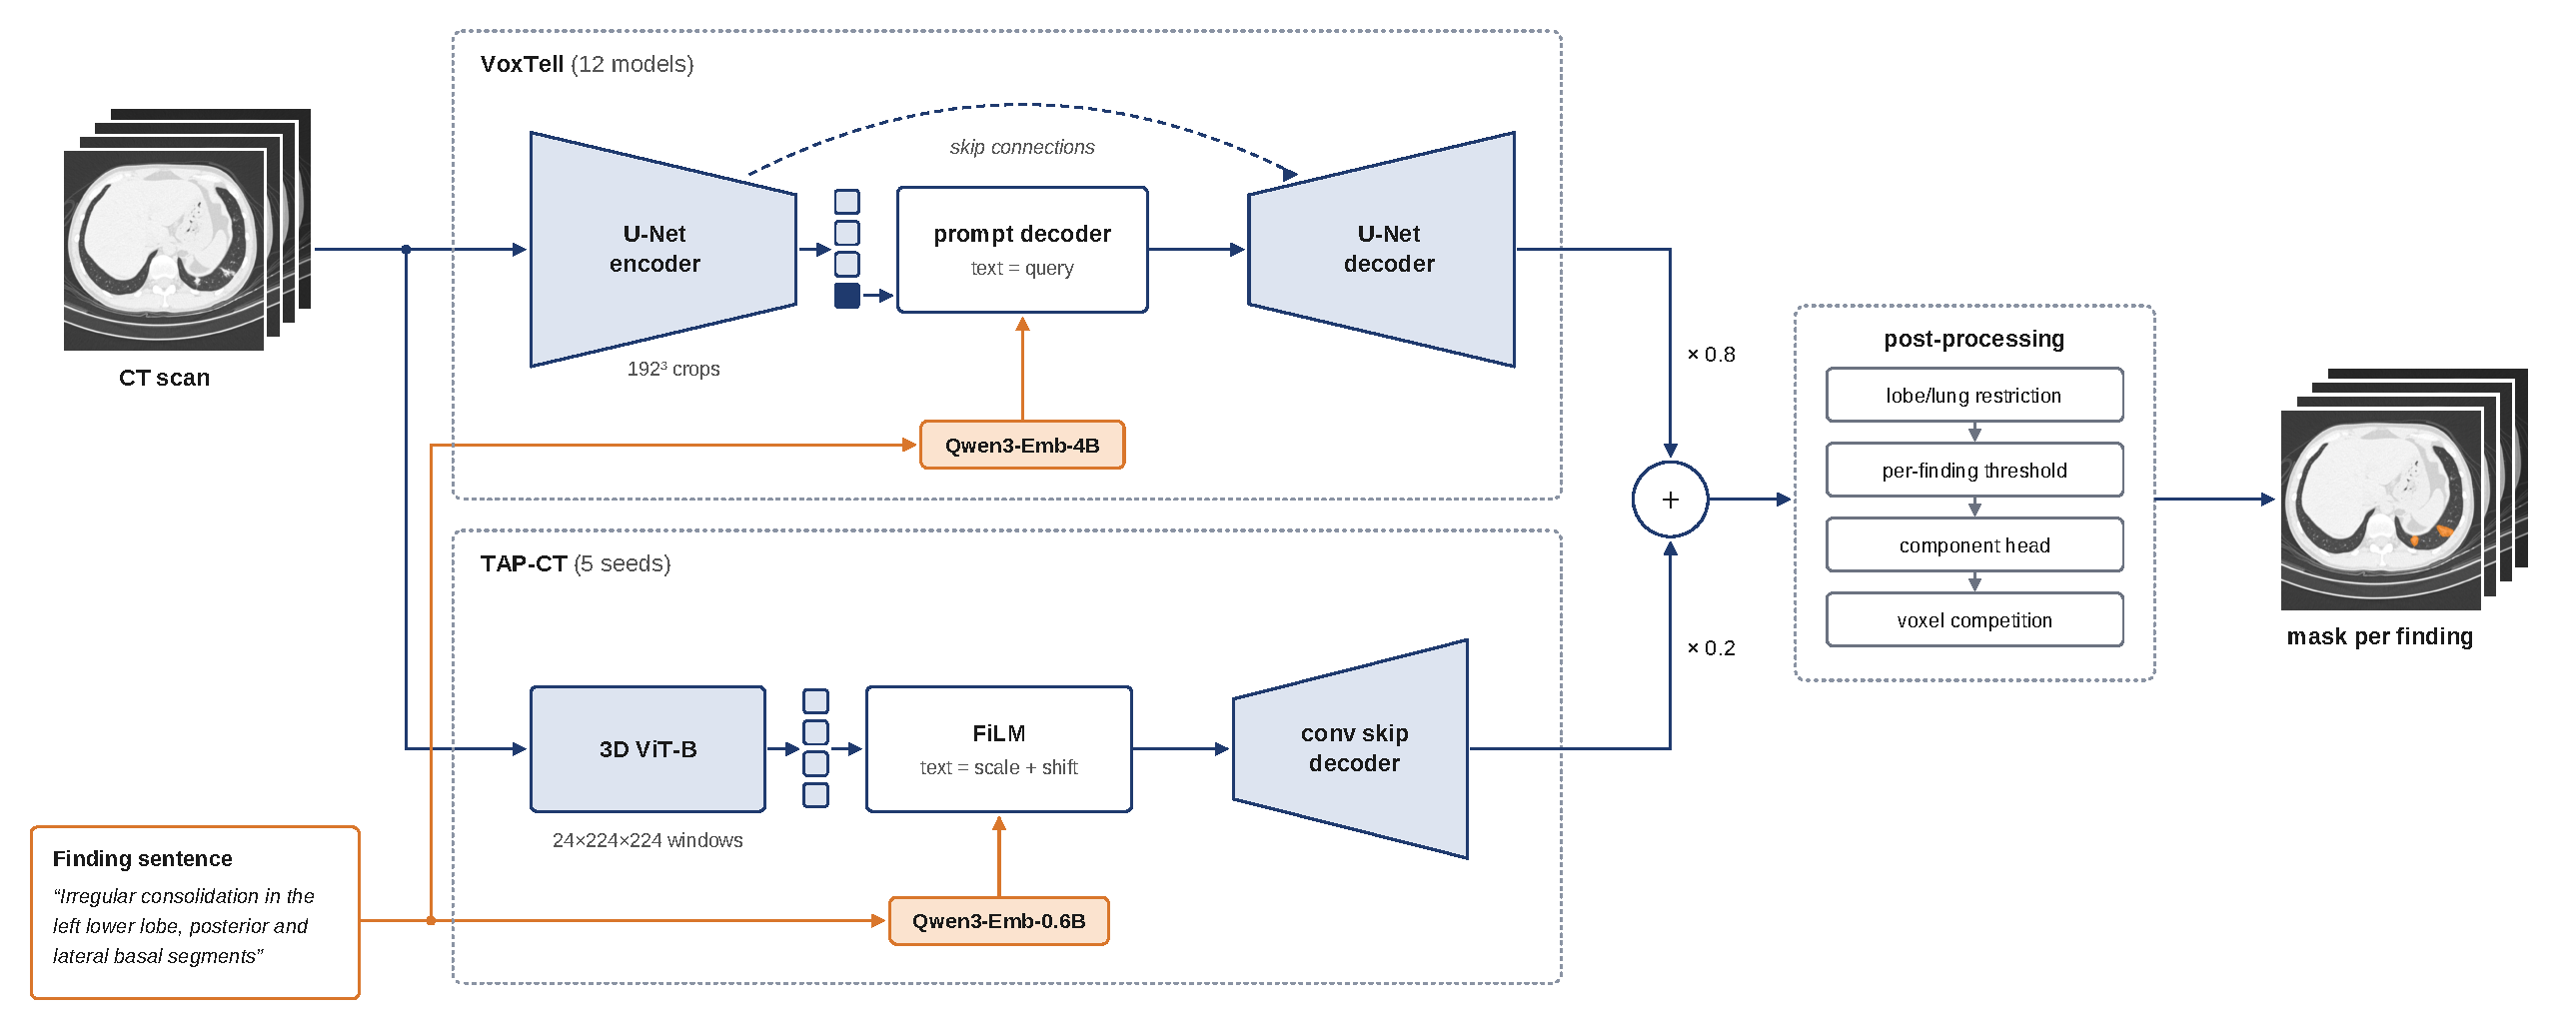
\includegraphics[width=\textwidth]{figures/appendix/team3_pipeline.pdf}
\caption{Team 3: twelve VoxTell models and five TAP-CT seeds, each conditioned on
the finding sentence, produce probability maps that are averaged per branch and
fused 0.8/0.2, followed by four post-processing steps.}
\label{fig:app-team3}
\end{figure*}
